\documentclass[sigconf,nonacm]{acmart}

% ACM Large 2-column per ECE 284 spec.
% If acmart is unavailable on Overleaf, replace the line above with:
% \documentclass[10pt,twocolumn]{article}
% and delete the \affiliation block below.

\settopmatter{printacmref=false, printfolios=false}
\renewcommand\footnotetextcopyrightpermission[1]{}
\pagestyle{plain}

\usepackage{graphicx}
\usepackage{booktabs}
\usepackage{hyperref}

\title{Multi-Modal Performance Sensing for Beach Volleyball: \\ Contextualizing Individual Performance Variability}

\author{Tristan Cooper}
\affiliation{%
  \institution{UC San Diego}
  \city{La Jolla}
  \state{CA}
  \country{USA}
}
\email{tmcooper@ucsd.edu}

\begin{document}

\begin{abstract}
Beach volleyball athletes experience large day-to-day performance variability that current tools cannot explain. Wearables report recovery scores without environmental context, weather apps miss court-level microclimate, and self-report compliance collapses under in-match cognitive load. This project builds a multi-modal sensing pipeline fusing wearable physiology (Oura Ring, Apple Watch), a custom courtside environmental node (ESP32 + BME280 + MLX90614 + mic), voice-based ecological momentary assessment, and computer-vision-derived performance metrics. The primary deliverable is a per-session factor-ranking analysis across 6--10 collected sessions, identifying which contextual streams best explain performance variation for an individual beach volleyball athlete. Contribution is sport-specific; methodological patterns are expected to inform related work in other sports.
\end{abstract}

\maketitle

%===================================================================
\section{Motivation}
%===================================================================

Athletes know some days they play well and others they do not. Isolating why is hard: recovery, environment, and mindset interact, and existing tools each measure one dimension in isolation.

\textbf{The problem.} Commercial wearables (WHOOP, Oura, Garmin) report readiness scores from overnight HRV and sleep staging but ignore same-day environmental load and subjective state. Weather apps report city-level conditions and miss court-level microclimate --- wind at Muir Field is reshaped by surrounding buildings, and sand surface temperature varies with grain size, moisture, and direct sun in ways ambient temperature cannot capture. Self-report instruments (EMA) are validated in sports psychology but compliance collapses under the cognitive burden of tapping through surveys mid-match. Computer-vision tools extract objective performance metrics with no context.

\textbf{The gap.} No existing system fuses recovery, environment, subjective state, and performance for an individual beach volleyball athlete. Each stream exists in isolation.

\textbf{Who benefits.} The immediate end user is the recreational or collegiate beach volleyball athlete who currently has no way to contextualize why a given session felt the way it did. The broader health relevance is exertional heat safety: beach volleyball is outdoors with no climate control, and early warning for heat strain requires exactly the physiological, environmental, and subjective fusion this pipeline produces.

%===================================================================
\section{Related Work}
%===================================================================

\textbf{Commercial wearable recovery.} WHOOP, Oura, and Garmin produce daily readiness scores from overnight biometrics. Validation studies show reasonable HRV and sleep accuracy under resting conditions, but these scores are not contextualized against same-day environmental or subjective state. % TODO: cite de Zambotti on Oura sleep validation if adding refs.

\textbf{Environmental monitoring in sport.} The FIVB enforces WBGT-based heat protocols at professional events and NATA publishes heat-illness position statements, but these rely on coarse point measurements and are absent from recreational and collegiate settings.

\textbf{Ecological momentary assessment.} EMA is well-validated in sports and behavioral health; voice-based capture has been proposed as a lower-burden alternative, and modern ASR (Whisper) with LLM extraction makes post-session processing practical.

\textbf{Wearables in beach volleyball.} Prior work exists but targets different questions. Marzano-Felisatti et al.\ (2024) applied an electronic performance tracking system to quantify physical-conditional performance of young male BV players, and the University of Sussex ``Wearables in Beach Volleyball'' project investigates IMU-based match load and event detection. Both focus on movement classification and training-load quantification from a single modality. Neither fuses physiological recovery state, environmental context, and subjective experience into a joint performance analysis. % TODO: add full citations.

\textbf{Gap.} No published system fuses recovery, environmental, subjective, and performance data at the level of the individual beach volleyball athlete.

%===================================================================
\section{Project Aim}
%===================================================================

\textbf{Primary aim.} Collect 6--10 synchronized multi-modal sessions on a single BV athlete (the author) and deliver a per-session factor-ranking analysis identifying which contextual streams best explain variation in performance.

\textbf{End user.} The athlete. Output is intended to be personally actionable --- \emph{``you played worse today because sleep debt and sand temperature were both elevated''} --- not a clinical or coaching product.

\textbf{Non-goals.} Not a predictive model for deployment. Not a cross-sport tool. Not clinically validated. Not recruiting additional subjects for v1.

%===================================================================
\section{Methodology}
%===================================================================

\begin{figure*}[t]
    \centering
    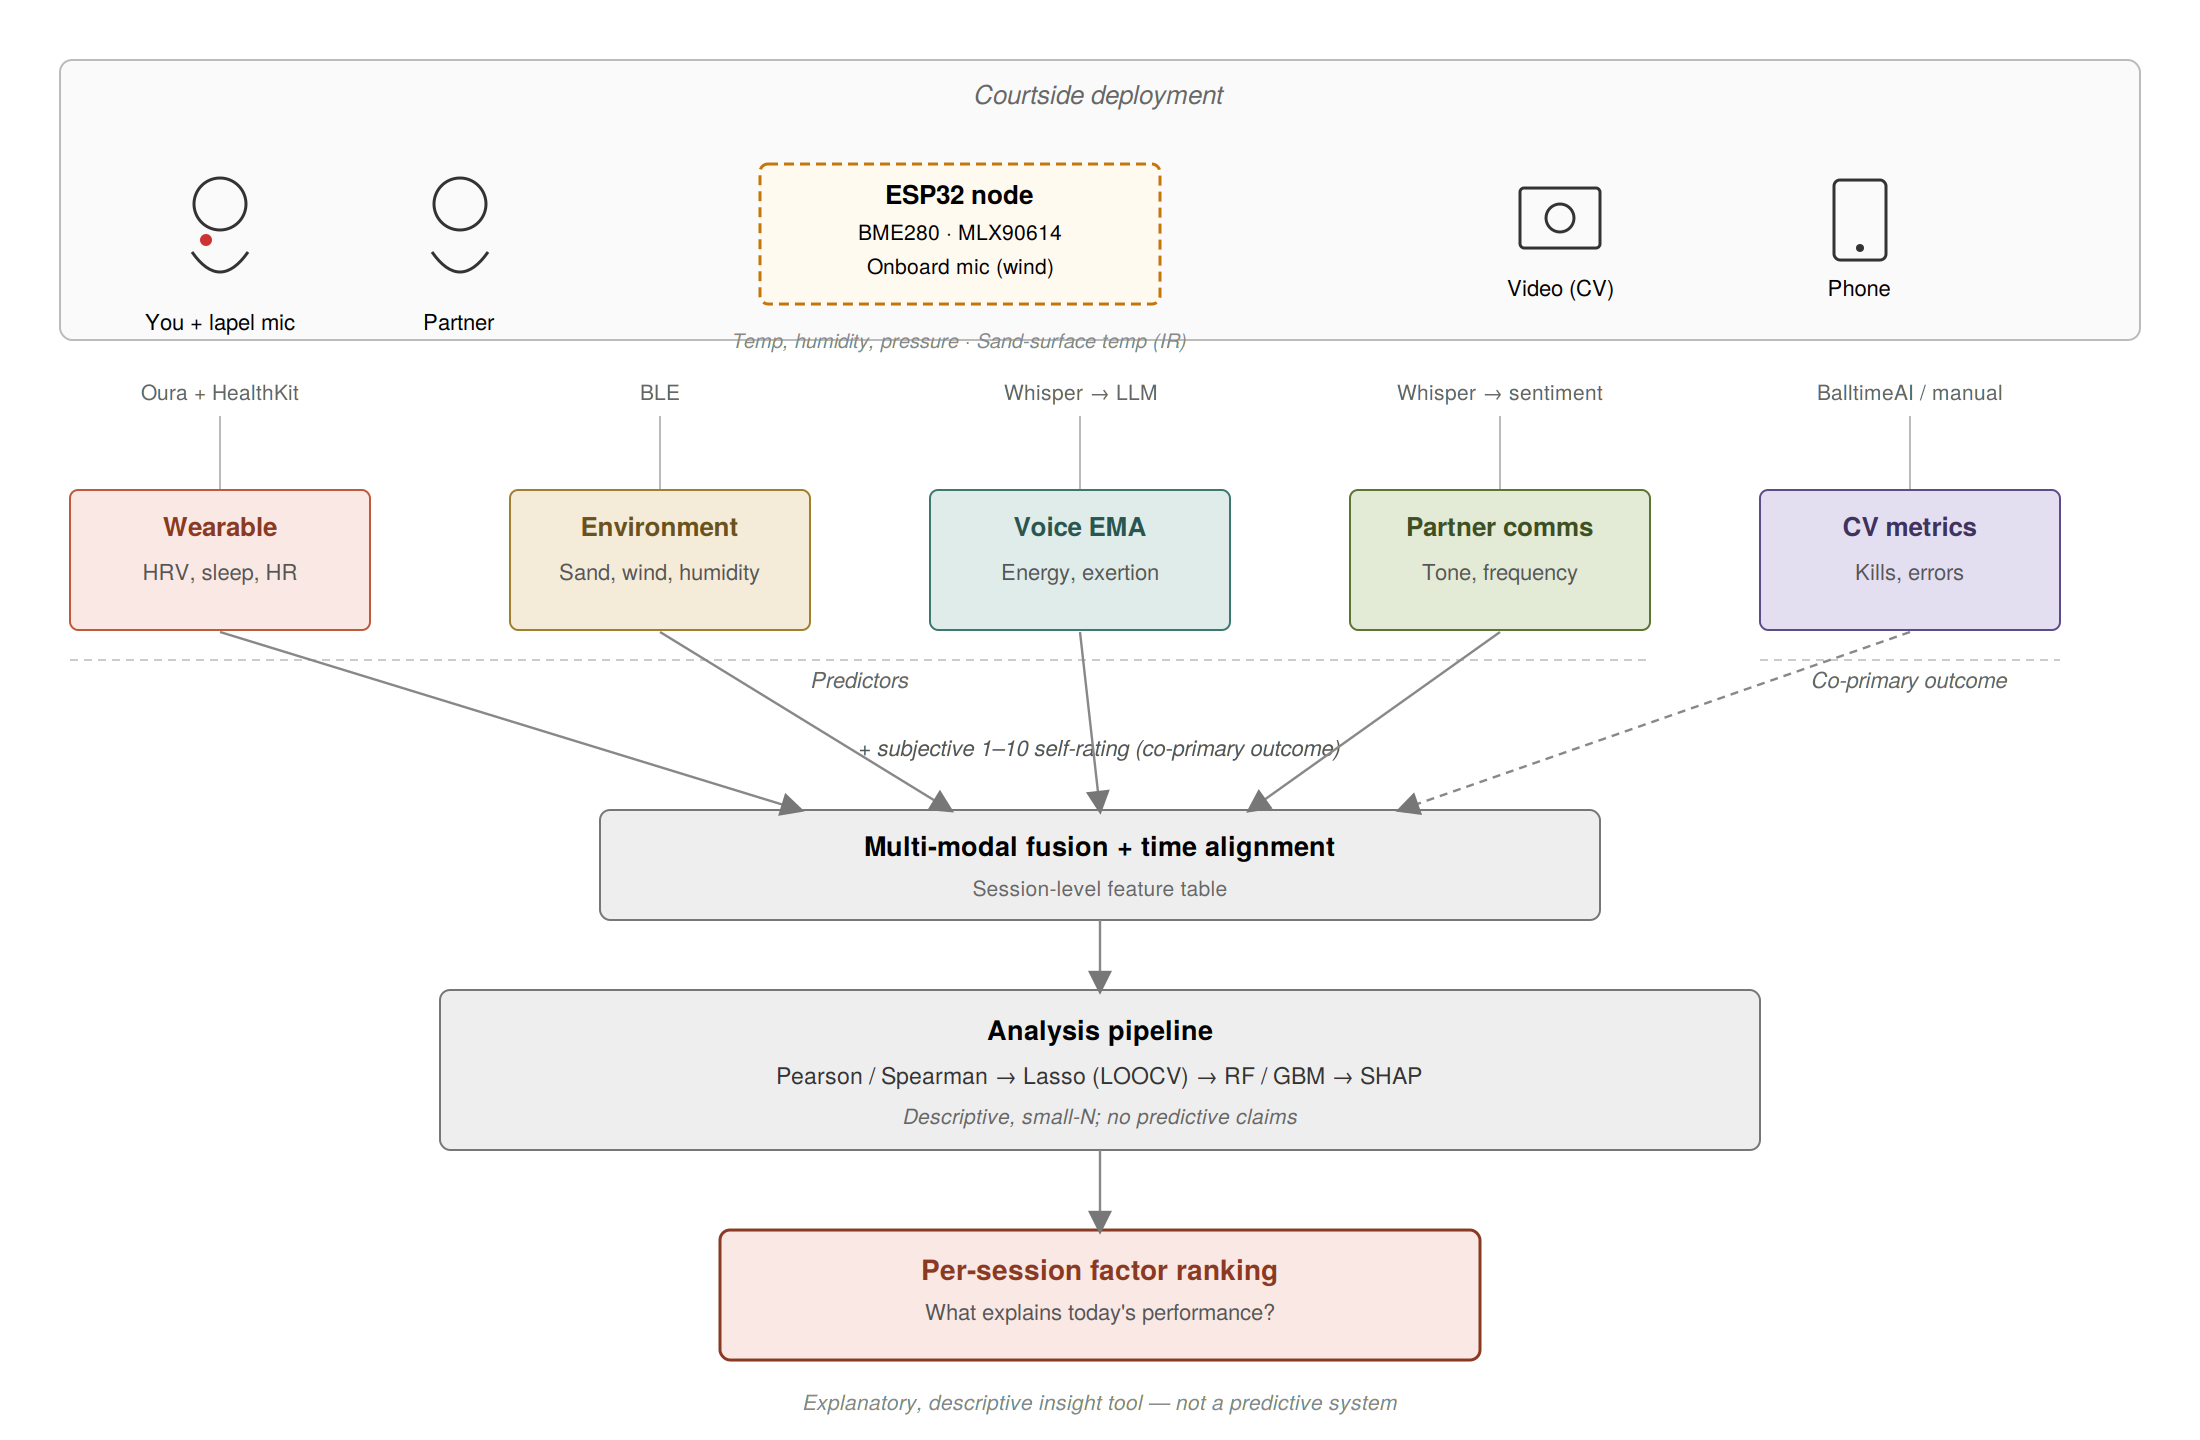
\includegraphics[width=0.92\textwidth]{system_architecture.png}
    \caption{System architecture. Five input streams are captured courtside and time-aligned into a session-level feature table. Four are predictors (wearable physiology, environment, voice EMA, partner communication) and one is a co-primary outcome (CV-based kill/error metrics), with a subjective 1--10 self-rating as the second co-primary outcome. The four-stage analysis pipeline produces per-session factor rankings as the primary deliverable.}
    \label{fig:architecture}
\end{figure*}

Figure~\ref{fig:architecture} summarizes the end-to-end system. The sections below detail each component.

\subsection{Data Streams}

\begin{itemize}
    \item \textbf{Wearable physiological.} Oura Ring (nightly HRV/RMSSD, sleep stages, body temperature deviation, readiness) via Oura API. Apple Watch (in-session HR at $\sim$1~Hz, between-set recovery) via HealthKit.
    \item \textbf{Environmental node.} ESP32 with BME280 (temp, humidity, pressure), MLX90614 (IR sand-surface temp), onboard microphone (audio amplitude as wind proxy). Tripod-mounted courtside, 1~Hz sampling, local SD-card logging.
    \item \textbf{Voice EMA + partner communication.} Wireless lapel microphone captures structured self-report between sets and passive partner communication during play. Post-session processing: Whisper ASR then LLM extraction against a structured rubric. Written partner consent required before any recording.
    \item \textbf{Performance outcome.} Per-set kill-minus-error differential via phone video (BalltimeAI where accessible, manual labeling otherwise) \textbf{and} a subjective 1--10 self-rating. Both are treated as co-primary outcomes.
\end{itemize}

\subsection{Data Handling and Preprocessing}

\begin{itemize}
    \item \textbf{Time alignment.} All streams aligned to the paired phone's NTP-synchronized clock. ESP32 receives time via BLE handshake at session start.
    \item \textbf{Unit of analysis.} Session-level features are the primary unit given small $N$; per-rally features are generated but reserved for stretch analysis.
    \item \textbf{Feature engineering.} Sleep debt (deviation from 7-day personal baseline), HRV z-score, heat stress index approximating WBGT from BME280 readings, partner communication rate per set, EMA-derived valence and confidence.
    \item \textbf{Storage.} Raw data per session stored in per-modality CSV/JSON. A unified session-level feature table is built downstream as input to analysis.
\end{itemize}

\subsection{Analysis Pipeline}

The analysis is exploratory and descriptive given $N \leq 10$. Four stages:

\begin{enumerate}
    \item Pearson and Spearman correlations of each feature against each outcome.
    \item Lasso regression with leave-one-out cross-validation for sparse feature selection.
    \item Random forest and gradient boosting on the Lasso-selected subset to capture interactions.
    \item SHAP values from the gradient boosting model for per-session factor rankings --- the primary deliverable.
\end{enumerate}

No $p$-values are reported as confirmatory. No model is released for deployment.

\subsection{Evaluation Criteria}

Because the output is a per-session explanation rather than a prediction, standard ML metrics (accuracy, AUC) do not apply. Evaluation is defined on four engineering criteria:

\begin{itemize}
    \item \textbf{Data completeness.} Fraction of sessions with all MVP streams captured end-to-end. Target $\geq 80\%$.
    \item \textbf{Time alignment accuracy.} Sub-second alignment between streams, validated by event markers at session start.
    \item \textbf{Ranking stability.} SHAP top-3 factor rankings should not change drastically with the addition of a single session. Measured via leave-one-session-out stability of the top-3 ranked features.
    \item \textbf{Face validity.} For each session, top-ranked factors are compared qualitatively to the athlete's own post-session recollection of why the session went well or poorly.
\end{itemize}

%===================================================================
\section{Timeline}
%===================================================================

\begin{itemize}
    \item \textbf{Week 4 (current, due Apr 20):} Project report. Hardware BOM finalized. Partner consent documented.
    \item \textbf{Week 5:} ESP32 node assembled and bench-validated. Oura API and HealthKit export pipelines operational on dummy data.
    \item \textbf{Week 6:} First pilot session. Debug sync, gaps, artifacts.
    \item \textbf{Week 7 (Project Update due):} $\geq 2$ sessions collected. System diagram + initial plots in update report.
    \item \textbf{Week 8:} Ramp to 2 sessions per week. Begin feature engineering.
    \item \textbf{Week 9:} Lock data collection. Run full analysis pipeline. Generate final figures.
    \item \textbf{Week 10 (final report Fri):} Writing, figure refinement, oral defense prep.
\end{itemize}

%===================================================================
\section{Scope Management and Risk}
%===================================================================

\textbf{MVP (floor).} Oura nightly data + Apple Watch in-session HR + BME280 environmental data + subjective 1--10 per-set rating + 6 sessions. End-to-end pipeline with reduced feature richness.

\textbf{Stretch.} MLX90614 sand-temperature, mic-based wind estimation, Whisper+LLM voice EMA pipeline, CV-based outcome via BalltimeAI, partner communication sentiment, teammate as second subject.

\textbf{Risks and mitigations.}
\begin{itemize}
    \item Hardware delays $\to$ MVP fallback stated above.
    \item Data loss / sync failures $\to$ redundant local logging, per-session validation before moving on.
    \item Weather cancellations $\to$ indoor practice sessions where environmental node is still informative.
    \item Small $N$ $\to$ all output framed as descriptive, no deployable model.
\end{itemize}

%===================================================================
\section{Conclusion and Generalization}
%===================================================================

The deliverable is a sport-specific instrument for an individual beach volleyball athlete. The methodological patterns --- time-aligning heterogeneous streams, small-$N$ feature ranking, face-validity evaluation against subjective recollection --- are not BV-specific and may inform related work in other sports, or adjacent populations where individual variability and environmental exposure both matter (heat-exposed workers, older adults at fall risk). Generalization is framed as future work, not a v1 claim.

%===================================================================
\section{AI Use Disclosure}
%===================================================================

AI tools (Claude) were used to (1) structure this report draft from the author's proposal slides. All technical content, experimental design, methodology choices, and timeline commitments were authored by the student. 

%===================================================================
% SUPPLEMENTAL PAGE
%===================================================================
\clearpage
\onecolumn
\section*{Supplemental: Classmate Feedback}

\subsection*{Classmate 1: Sehaj Dhillon --- passive behavioral monitoring for mental health support}

\textbf{Feedback.} Sehaj affirmed the gap framing came through clearly: many individual metrics can be measured during athletic performance but no system fuses them for joint insight. Three points: (1) the proposal read sport-agnostic --- does the system generalize across sports, or is it beach-specific, and does supporting data exist for either case? (2) Is data already collected or is self-collection still planned? (3) The slide still listed ``Technique TBD'' for ML analysis --- is the plan comparative methods or a committed approach?

\textbf{Response (incorporated).} Section~3 now locks the project to beach volleyball as a sport-specific tool, with generalization scoped to Section~8 as future work. Section~5 timeline makes explicit that no prior data exists and all sessions are collected during Weeks 6--9. Section~4.3 commits to a specific four-stage analysis pipeline (correlations $\to$ Lasso/LOOCV $\to$ RF/GBM $\to$ SHAP) rather than a comparative methods study.

\subsection*{Classmate 2: Foster --- smartphone eye-chart visual acuity screening}

\textbf{Feedback.} Foster raised five points: (1) how will the heterogeneous context data be organized, cleaned, and tidied? (2) How will each stream be preprocessed to feed into the ML model? (3) Given the small sample size, how will results be interpreted? (4) Is the hardware actually available to gather all proposed inputs, or would existing datasets be a better fit to focus on analysis and modeling? (5) What evaluation metrics will critique the agent's outputs, given that even paid private coaches operate on limited data? He also noted the personal-life relevance of the project as a strength.

\textbf{Response (incorporated).} A new Section~4.2 (Data Handling and Preprocessing) explicitly describes per-stream format, time alignment to the phone's NTP clock, unit of analysis, feature engineering, and storage. A new Section~4.4 (Evaluation Criteria) defines four evaluation axes --- data completeness, time alignment accuracy, SHAP ranking stability, and face validity against the athlete's own recollection --- to replace the ML-metric framing that does not apply to a per-session explanation output. On datasets: self-collection is retained because no existing public dataset captures the full multi-modal stack required for this analysis; small-$N$ interpretation risk is addressed by framing all output as descriptive rather than predictive (Section~4.3).

\subsection*{Classmate 3: Jinglin Zheng --- context-aware health behavior agent}

\textbf{Feedback.} Jinglin found the motivation clear, related work thorough, and the data processing pipeline technically deep and innovative. The main concern was scope breadth: hardware data collection + software processing + ML modeling may be hard to complete in a month. He also noted that target features and evaluation criteria were not clearly defined and would need to be specified in subsequent iterations.

\textbf{Response (incorporated).} The MVP/Stretch split in Section~6 directly addresses scope: the floor commitment (Oura + Apple Watch + BME280 + subjective rating + 6 sessions) delivers an end-to-end pipeline within the timeline, with voice EMA, CV-based outcome, and the full ESP32 sensor complement as stretch goals attempted only after MVP data collection is locked. Target features are now enumerated in Section~4.2 (feature engineering bullet) and evaluation criteria are explicit in Section~4.4.

\end{document}